%--------------------------------------------------
\section{Modelo de entidades del negocio}

\begin{figure}[htbp!]
		\centering
			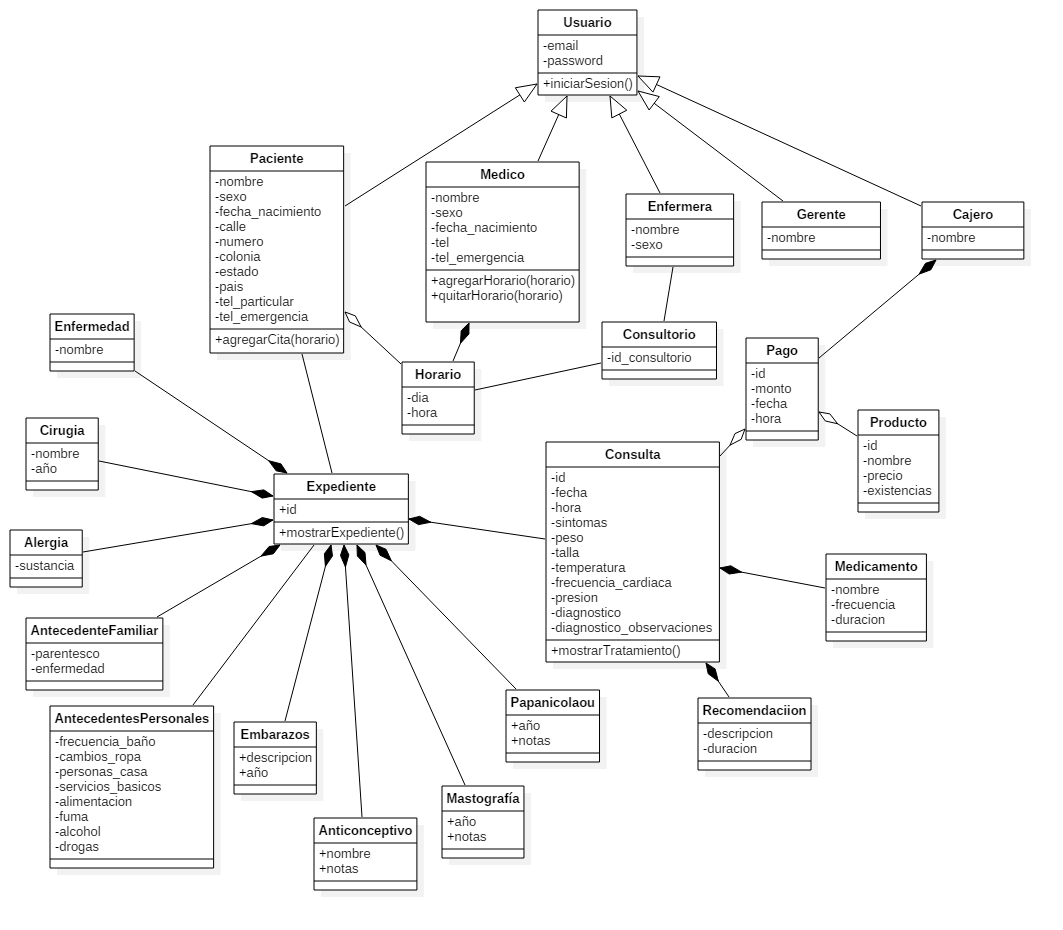
\includegraphics[width=1.1\textwidth]{images/Diagrama_clases}
		\caption{Diagrama de clases.}
	\end{figure}

\newpage

%--------------------------------------------------
\section{Descripción de atributos}



\subsection{Atributos de Usuario:}
\begin{description}
\item[email: ]Correo electrónico válido con el que se identifica al paciente.
\item[password: ]Cadena de caracteres para que el paciente ingrese al sistema.
\end{description}

\subsection{Atributos de Paciente:}
\begin{description}
\item[nombre: ]Nombre del paciente.
\item[sexo: ]Carácter que indica el género del paciente [H/M].
\item[fecha\_nacimiento: ]Fecha en formato DD/MM/YY de nacimiento del paciente.
\item[calle: ]Nombre de calle de domicilio de paciente.
\item[numero: ]Número de domicilio del paciente.
\item[colonia: ]Colonia donde se ubica domicilio de paciente.
\item[estado: ]Estado donde reside el paciente.
\item[pais: ]País donde reside el paciente.
\item[tel\_particular: ]Teléfono para contactar al paciente.
\item[tel\_emergencias: ]Teléfono en caso de emergencia del paciente.
\end{description}

\subsection{Atributos de Médico:}
\begin{description}
\item[nombre: ]Nombre del médico.
\item[sexo: ]Caracter que indica el género del médico [H/M].
\item[fecha\_nacimiento: ]Fecha en formato DD/MM/YY de nacimiento del médico.
\item[tel\_particular: ]Teléfono para contactar al médico.
\item[tel\_emergencias: ]Teléfono en caso de emergencia.
\end{description}

\subsection{Atributos de Enfermera:}
\begin{description}
\item[nombre: ]Nombre de enfermera.
\item[sexo: ]Caracter que indica el género del enfermero o enfermera [H/M].
\end{description}

\subsection{Atributos de Gerente:}
\begin{description}
\item[nombre: ]Nombre del gerente.
\end{description}

\subsection{Atributos de Cajero:}
\begin{description}
\item[nombre: ]Nombre del cajero.
\end{description}

\subsection{Atributos de Horario:}
\begin{description}
\item[horario: ]Horario de consulta.
\item[fecha: ]Fecha de consulta.
\end{description}

\subsection{Atributos de Consultorio:}
\begin{description}
\item[id: ]Identificador o número de consultorio.
\end{description}

\subsection{Atributos de Enfermedad:}
\begin{description}
\item[nombre: ]Nombre de la enfermedad.
\end{description}

\subsection{Atributos de Cirugía:}
\begin{description}
\item[nombre: ]Nombre descriptivo de la cirugía.
\item[año: ]Año en el que fue practicada la cirugía.
\end{description}

\subsection{Atributos de Alergia:}
\begin{description}
\item[sustancia: ]nombre de la sustancia a la que es alérgico el paciente.
\end{description}

\subsection{Atributos de AntecedenteFamiliar:}
\begin{description}
\item[parentesco: ]Parentesco con el paciente de la persona que sufre el antecedente.
\item[enfermedad: ]Enfermedad padecida por el familiar.
\end{description}

\subsection{Atributos de AntecedentesPersonales:}
\begin{description}
\item[frecuencia\_baño: ]Número de veces a la semana en las que se baña el paciente.
\item[cambios\_ropa: ]número de veces que el paciente cambia de ropa en una semana.
\item[personas\_casa: ]número de personas que residen junto con el paciente.
\item[servicios\_basicos: ]Lista de servicios básicos (Agua, drenaje,luz...) con los que cuenta el paciente.
\item[alimentacion: ]Indica si la alimentación es buena, regular o mala.
\item[fuma: ]si/no fuma.
\item[alcohol: ]si/no toma alcohol.
\item[drogas: ]Lista de drogas que ingiere el paciente.
\end{description}

\subsection{Atributos de Embarazo:}
\begin{description}
\item[descripción: ]Descripción del evento de embarazo.
\item[año: ]Año del evento.
\end{description}

\subsection{Atributos de Anticonceptivo:}
\begin{description}
\item[nombre: ]Nombre del anticonceptivo que utiliza.
\item[notas: ]Notas adicionales.
\end{description}

\subsection{Atributos de Mastografía}
\begin{description}
\item[año: ]Año en que se le practicó mastografía.
\item[notas: ]Notas adicionales.
\end{description}

\subsection{Atributos de Papanicolaou}
\begin{description}
\item[año: ]Año en que se le practicó papanicolaou.
\item[notas: ]Notas adicionales.
\end{description}

\subsection{Atributos de Consulta:}
\begin{description}
\item[id: ]Identificador numérico de consulta.
\item[fecha: ]Fecha de consulta.
\item[hora: ]Hora de consulta.
\item[síntomas: ]Síntomas presentados por paciente
\item[peso: ]Peso en Kg  del paciente.
\item[talla: ]Talla en cm del paciente.
\item[temperatura: ]Temperatura en $\degree$C del paciente.
\item[frecuencia\_cardiaca: ]Frecuencia cardíaca del paciente medida en pulsaciones por minuto.
\item[presión: ]Presión arterial del paciente medida en mmHg.
\item[diagnostico: ]Diagnóstico concludo por el médico.
\item[diagnostico\_observaciones: ]Observaciones médicas sobre el diagnóstico dado.
\end{description}

\subsection{Atributos de Recomendación:}
\begin{description}
\item[descripción: ]Descripción de la recomendación médica.
\item[duración: ]Duración de la recomendación.
\end{description}

\subsection{Atributos de Medicamento:}
\begin{description}
\item[nombre: ]Nombre del medicamento recetado.
\item[frecuencia: ]Frecuencia con la que se debe ingerir el medicamento.
\item[duracion: ]Duración de la toma del medicamento.
\end{description}

\subsection{Atributos de Pago}
\begin{description}
\item[id: ]Identificador numérico de pago.
\item[monto: ]Monto total de dinero pagado.
\item[fecha: ]Fecha de la transacción.
\item[hora: ]Hora de la transacción.
\end{description}

\subsection{Atributos de Producto}
\begin{description}
\item[id: ]Identificador numérico del producto.
\item[nombre: ]Nombre del producto.
\item[precio: ]Precio en MXN del producto.
\item[existencias: ]Cantidad de unidades que se tienen disponibles.
\end{description}

